\documentclass{article}

\usepackage{amsmath, amsthm, amssymb, amsfonts}
\usepackage{thmtools}
\usepackage{graphicx}
\usepackage{setspace}
\usepackage{geometry}
\usepackage{float}
\usepackage{tikz}
\usetikzlibrary{shapes}
\usepackage{float}
\usepackage{hyperref}
\usepackage[utf8]{inputenc}
\usepackage[english]{babel}
\usepackage{framed}
\usepackage[dvipsnames]{xcolor}
\usepackage{tcolorbox}
\usepackage[backend=biber,style=ieee]{biblatex}
\addbibresource{references.bib}

\colorlet{LightGray}{White!90!Periwinkle}
\colorlet{LightOrange}{Orange!15}
\colorlet{LightGreen}{Green!15}

\newcommand{\HRule}[1]{\rule{\linewidth}{#1}}

\declaretheoremstyle[name=Theorem,]{thmsty}
\declaretheorem[style=thmsty,numberwithin=section]{theorem}
\tcolorboxenvironment{theorem}{colback=LightGray}

\declaretheoremstyle[name=Proposition,]{prosty}
\declaretheorem[style=prosty,numberlike=theorem]{proposition}
\tcolorboxenvironment{proposition}{colback=LightOrange}

\declaretheoremstyle[name=Principle,]{prcpsty}
\declaretheorem[style=prcpsty,numberlike=theorem]{principle}
\tcolorboxenvironment{principle}{colback=LightGreen}

\setstretch{1.2}
\geometry{
    textheight=9in,
    textwidth=5.5in,
    top=1in,
    headheight=12pt,
    headsep=25pt,
    footskip=30pt
}

% ------------------------------------------------------------------------------

\begin{document}

% ------------------------------------------------------------------------------
% Cover Page and ToC
% ------------------------------------------------------------------------------

\title{ \normalsize \textsc{}
		\\ [2.0cm]
		\HRule{1.5pt} \\
		\LARGE \textbf{\uppercase{Final Project Proposal}
		\HRule{2.0pt} \\ [0.6cm] \LARGE{Incompressible Navier-Stokes for Lid-Driven Cavity using SIMPLE Method} \vspace*{10\baselineskip}}
		}
\date{}
\author{\textbf{Author} \\ 
		Noah Reef \\
		UT Austin \\
		Fall 2025}

\maketitle
\newpage

\tableofcontents
\newpage

% ------------------------------------------------------------------------------

\section{Introduction}
 The lid-driven cavity flow has long served as a canonical benchmark for the numerical
solution of the incompressible Navier–Stokes equations. Despite its geometric simplicity,
the problem exhibits complex flow features such as strong recirculation, corner vortices,
and increasing sensitivity to numerical discretization as the Reynolds number increases.
Consequently, it has been widely used to assess the accuracy, stability, and efficiency of
numerical methods for incompressible flows. The problem can be formulated as solving the Incompressible Navier-Stokes,
\begin{align}
  \nabla \cdot \pmb{u} &= 0 \\
  \frac{\partial \pmb{u}}{\partial t} + \pmb{u} \cdot \nabla \pmb{u} &= -\nabla p + \frac{1}{\text{Re}} \nabla^2 \pmb{u}
\end{align}
with $u(0,y,t) = u(x,0,t) = u(L,y,t) = 0$, $v(0,y,t) = v(x,0,t) = v(L,y,t) = v(x,L,t) = 0$, and $u(x,L,t) = 1$.
\begin{figure}[H]
  \centering
      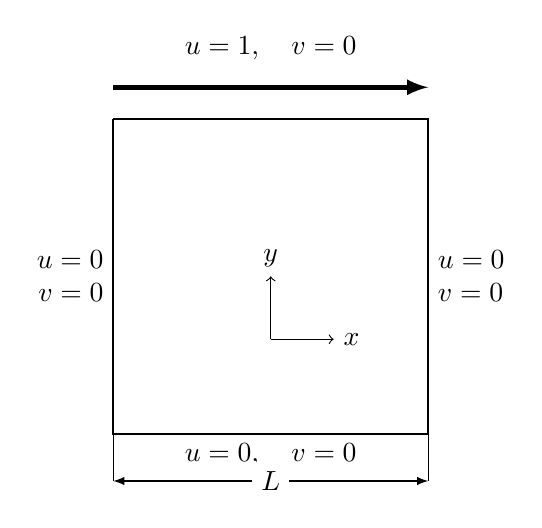
\begin{tikzpicture}[scale=4]
    % 1. Define the Square Domain
    % Draw the three stationary walls (Left, Bottom, Right)
    \draw[thick] (0,1) -- (0,0) -- (1,0) -- (1,1) -- (0,1);
    
    % Draw the moving lid (Top) - usually thicker or emphasized
    \draw[ultra thick, ->, >=latex] (0,1.1) -- (1,1.1) node[midway, above=2mm] {$u = 1, \quad v = 0$};

    % 2. Add Boundary Condition Labels
    % Left Wall
    \node[left, align=right] at (0,0.5) {$u=0$\\$v=0$};
    % Right Wall
    \node[right, align=left] at (1,0.5) {$u=0$\\$v=0$};
    % Bottom Wall
    \node[below, align=center] at (0.5,0) {$u=0, \quad v=0$};

    % 3. Coordinate System (Optional)
    \draw[->] (0.5, 0.3) -- (0.7, 0.3) node[right] {$x$};
    \draw[->] (0.5, 0.3) -- (0.5, 0.5) node[above] {$y$};

    % --- Dimension Line for L ---
    % Draw tick lines extending down from the corners
    \draw[thin] (0,0) -- (0,-0.15);
    \draw[thin] (1,0) -- (1,-0.15);
    % Draw the dimension line with arrows and label in the middle
    % fill=white makes the label readable over the line
    \draw[thin, <->, >=latex] (0,-0.15) -- (1,-0.15) node[midway, fill=white] {$L$};

\end{tikzpicture}
  \caption{Lid-Driven Cavity}
  \label{fig:Lid-Driven}
\end{figure}
The depiction of the problem can be seen in Figure \ref{fig:Lid-Driven}.  

\section{Related Work}

Many benchmark studies compare results to \cite{ghia1982high}, who utilized a multi-grid strategey to a strongly implicit method to discretize the stream function and vorticity Navier-Sotkes equations. They use a grid meshs up to $257 \times 257$ number of grid points and Reynold's numbers up to $10,000$. 

Other numerical approaches, such as in \cite{barragy1997streamfunction} used a $p$-type finite-element scheme on $257 \times 257$ fine element mesh and yielded highly accurate solutions for Reynold's numbers up to $12,500$. 

Further advances in solution accuracy were achieved using spectral methods. In \cite{botella1998benchmark} they use Chebyshev spectral discretizations, obtaining highly accurate spectral solutions for the cavity flow with a maximum grid mesh of $N=160$ for Reynold's numbers up to $9,000$ 

In \cite{wright1995efficient} they applied the Block Implicit Multigrid Method (BIMM) to the SMART and QUICK discretizations, yielding results on a $1024 \times 1024$ grid mesh for $\text{Re} \leq 1,000$. 

In addition to these classical approaches, pressure-based methods formulated in primitive variables have become widely used due to their flexibility and robustness. The Semi-Implicit Method for Pressure-Linked Equations (SIMPLE) remains one of the most common pressure–velocity coupling strategies for incompressible flows. 
\section{Problem Formulation}
We can express the following problem component-wise, taking $\pmb{u} = (u,v)$, and yield
\begin{align}
  \frac{\partial u}{\partial x} + \frac{\partial v}{\partial y} &= 0 \\
  \frac{\partial u}{\partial t} + \left(\frac{\partial u^2}{\partial x} + \frac{\partial uv}{\partial y}\right) &= - \frac{\partial p}{\partial x} + \frac{1}{\text{Re}}\left(\frac{\partial^2 u}{\partial x^2} + \frac{\partial^2 u}{\partial y^2}\right) \\
  \frac{\partial v}{\partial t} + \left(\frac{\partial v^2}{\partial y} + \frac{\partial uv}{\partial x}\right) &= - \frac{\partial p}{\partial y} + \frac{1}{\text{Re}}\left(\frac{\partial^2 v}{\partial x^2} + \frac{\partial^2 v}{\partial y^2}\right)  
\end{align}

\subsection{Staggered-Grid Discretization}
\begin{figure}[H]
  \centering
      \begin{tikzpicture}[scale=4]
    % 1. Define the Square Domain
    % Draw the three stationary walls (Left, Bottom, Right)
    \draw[thick] (0,1) -- (0,0) -- (1,0) -- (1,1) -- (0,1);
    
    
    \draw[thick, ->, >=latex] (-0.5,0.5) -- (-0.1,0.5);
    \draw[thick, ->, >=latex] (0.4,0.5) -- (0.8,0.5);
    \draw[thick, ->, >=latex] (0.4,1.1) -- (0.8,1.1);
    \draw[thick, ->, >=latex] (0.4,-0.15) -- (0.8,-0.15);
    \draw[thick, ->, >=latex] (1.1,0.5) -- (1.5,0.5);

    % --- Dimension Line for L ---
    % Draw tick lines extending down from the corners
    \draw[thick, ->, >=latex] (0,-0.4) -- (0,0);
    \draw[thick, ->, >=latex] (1,-0.4) -- (1,0);
    \draw[thick, ->, >=latex] (1,1) -- (1,1.4);
    \draw[thick, ->, >=latex] (0,1) -- (0,1.4);
    
    \draw (0,0.5) circle (0.8pt);
    \draw (1,0.5) circle (0.8pt);

    \node[above, align=center] at (0.6,0.5) {$u_{i,j}$};
    \node[above, align=center] at (-0.4,0.5) {$u_{i,j-1}$};
    \node[above, align=center] at (1.2,0.5) {$u_{i,j+1}$};
    \node[above, align=center] at (0.5,1.1) {$u_{i-1,j}$};
    \node[above, align=center] at (0.5,-0.15) {$u_{i+1,j}$};

    \node[left, align=center] at (0,1.2) {$v_{i-1,j}$};
    \node[left, align=center] at (0,-0.1) {$v_{i,j}$};
    \node[right, align=center] at (1,-0.1) {$v_{i,j+1}$};
    \node[right, align=center] at (1,1.2) {$v_{i-1,j+1}$};
    
    \node[above, align=center] at (0,0.5) {$p_{i,j}$};
    \node[below, align=center] at (1,0.5) {$p_{i,j+1}$};
  
    
\end{tikzpicture}
  \caption{Staggered Grid Discretization}
  \label{fig:Disc}
\end{figure}

The staggered grid discretization can be seen in Figure \ref{fig:Disc}, and we can rewrite the Incompressible Naiver-Stokes for the $u$-component as, 
\begin{align*}
  \left( \frac{\partial u}{\partial t} \right)_i^n&= \frac{u_{i,j}^{n+1} - u_{i,j}^n}{k} \\
  \left(  \frac{\partial u^2}{\partial x} \right)_i^n&= \frac{\left(\frac{u_{i,j} + u_{i,j+1}}{2}\right)^2 - \left(\frac{u_{i,j-1} + u_{i,j}}{2}\right)^2 }{h_x} \\
  \left(  \frac{\partial uv}{\partial y} \right)_i^n &= \frac{\left(\frac{u_{i,j} + u_{i-1,j}}{2}\right)\left(\frac{v_{i-1,j}+v_{i-1,j+1}}{2}\right) - \left(\frac{u_{i,j} + u_{i+1,j}}{2}\right) \left(\frac{v_{i,j} + v_{i,j+1}}{2}\right)}{h_y} \\
  \left(\frac{\partial p}{\partial x}\right)_i^n &= \frac{p_{i,j+1} - p_{i,j}}{h_x} \\
  \left(\frac{\partial^2 u}{\partial x^2} + \frac{\partial^2u}{\partial y^2}\right)_i^n &= \frac{u_{i,j+1} - 2u_{i,j} + u_{i,j-1}}{h_x^2} + \frac{u_{i-1,j} - 2u_{i,j} + u_{i+1,j}}{h_y^2}
\end{align*}
note that we can do a similar discretization for the $v$-component.

\section{Goals}
For this project we aim to implement a solver using the Semi-Implicit Method for Pressure-Linked Equations in Python. We hope to obtain results similar to that achieved in \cite{mathworks_simple}

\section{Timeline}
\begin{table}[H]
    \centering
    \begin{tabular}{| m{5cm} | p{8cm} |}
        \hline
         11/3 - 11/7 & Perform Additional Literature Review\\
        \hline
         11/9 - 11/14  & Desing intital solver code, perform necessary debugging, etc. \\
         \hline
         11/16 - 11/21 & Additional necessary debugging and error analysis, begin write-up\\
         \hline
         12/1 - 12/5 & Finalize results and write-up. \\
         \hline
    \end{tabular}
    \caption{Proposed Timeline}
    \label{tab:placeholder}
\end{table}

\printbibliography[title={References}, heading=bibintoc]


\end{document}

